\documentclass[a4paper, 11pt]{article}
\usepackage[title]{appendix}
\usepackage{comment} % enables the use of multi-line comments (\ifx \fi) 
\usepackage{fullpage} % changes the margin
\usepackage{graphicx} % include graphics
\usepackage{subcaption} % allows for sub captions
\usepackage{indentfirst} %indents first sentence of a paragraph
\usepackage[utf8]{inputenc}
\usepackage[fleqn]{amsmath}
\usepackage{listing}
\usepackage{gensymb}
\usepackage{amssymb}
\usepackage{mathtools}
\usepackage{array}
\usepackage{hyperref}
\usepackage[T1]{fontenc}
\usepackage[margin=1in]{geometry}
\usepackage{lmodern}
\usepackage{tabularx}
\usepackage{fancyhdr}
\usepackage{graphicx}
\graphicspath{{images/}}
\usepackage{minted}
\usepackage{cleveref}
\usepackage{xcolor}
\usepackage{listings}
\usepackage{dirtree}
\usepackage{stackengine}
%\documentclass[tikz,border=10pt]{standalone}
\usepackage[linguistics]{forest}
\usepackage[titles]{tocloft}
\usepackage{pdfpages}

\definecolor{darkscarlet}{rgb}{0.34, 0.01, 0.1}
\definecolor{ultramarineblue}{rgb}{0.25, 0.4, 0.96}
\definecolor{alizarin}{rgb}{0.82, 0.1, 0.26}
\definecolor{cadmiumgreen}{rgb}{0.0, 0.42, 0.24}
\definecolor{desertsand}{rgb}{0.93, 0.79, 0.69}
\definecolor{weborange}{rgb}{1,0.68,0}
\definecolor{frenchplum}{rgb}{0.51,0.078,0.33}

% The following is a dummy icon command
\newcommand\myicon[1]{{\color{#1}\rule{2ex}{2ex}}}
% If you have actual icon images, use \includegraphics to include them
% If you are generating them, put in the appropriate code for them here
% now we make a command for a folder/file which inserts the icon and its label
% adjust this as needed. If you only have 2 icons, then you could create
% a \myfile and \myfolder command with the icon fixed.
\newcommand{\myfolder}[2]{\myicon{#1}\ {#2}}

\setminted{fontsize=\small,baselinestretch=0.75}

\usepackage{listings}
\usepackage{caption}

\lstset{language=C, keywordstyle={\bfseries \color{black}}}

% defines algorithm counter for chapter-level
\newcounter{nalg}[section]

%defines appearance of the algorithm counter
\renewcommand{\thenalg}{\thesection .\arabic{nalg}}

% defines a new caption label as Algorithm x.y
\DeclareCaptionLabelFormat{algocaption}{Pseudocode \thenalg}

% defines the algorithm listing environment
\lstnewenvironment{pseudocode}[1][] {
    \refstepcounter{nalg}  % increments algorithm number
    \captionsetup{font=normalsize, labelformat=algocaption, labelsep=colon}
    \lstset{
    breaklines=true,
    language=C++,
    frame=tb,
    tabsize=2,
    showstringspaces=false,
    numbers=left,
    %upquote=true,
    commentstyle=\color{green},
    keywordstyle=\color{desertsand},
    keywords={operation, class},
    stringstyle=\color{cadmiumgreen},
    basicstyle=\small\ttfamily, % basic font setting
    emph={class,operation,dereference,reference_to,encrypt,decrypt,attribute,assign,return,call,if,else,is,while,open,instantiate,inherits,from},
    emphstyle={\color{blue}},
    % keyword highlighting
    classoffset=1, % starting new class
    otherkeywords={>,<,.,;,-,!,=,~,:,String,Integer,Bytes,Boolean,PatientRecord,VisitRecord,QueryMap,AdministrativeSuite,true,false},
    morekeywords={>,<,.,;,-,!,=,~,:,String,Integer,Bytes,Boolean,PatientRecord,VisitRecord,QueryMap,AdministrativeSuite,true,false},
    keywordstyle=\color{frenchplum},
    classoffset=0,
    xleftmargin=.04\textwidth,
    #1
}
}{}

\begin{document}
%Header-Make sure you update this information!!!!
% \noindent
% \large\textbf{Assignment 03} \hfill Due Date: 30 Nov 2020 \\
% \normalsize EN.605.601: Foundations of Software Engineering \\
% Group Members: Sabbir Ahmed, Kristy Cappelli, \& Chuck Norris \\
% Assignment Leader: Sabbir Ahmed

\begin{titlepage}
   \begin{center}
       \vspace*{1cm}

        \huge
        \textbf{GoodMead Hospital Management System}

        \vspace{0.5cm}

        \LARGE
        From Analysis to Design and Architecture

        \vspace{0.5cm}        
        \large
        \textbf{Sabbir Ahmed, Kristy Cappelli, \& Chuck Norris}

        \vfill

        \includegraphics[width=0.4\textwidth]{GoodMeadLogo.png}

        EN.605.601: Foundations of Software Engineering\\
        Johns Hopkins University\\
        \today

   \end{center}
\end{titlepage}


\tableofcontents

\newpage

\section{Introduction}

The purpose of this deliverable is to document the analysis, design and system architecture of a use case of \textbf{GoodMead: A Hospital Management System (HMS)}. The use case chosen was "Doctor Updates Patient Records" replicated below.
%\subsubsection{Figure: Use Case Diagram}
\begin{figure}[!htb]
    \centering
        \includegraphics[width=0.8\textwidth]{UseCase.jpg}
    \caption{Use Case Diagram}\label{fig:use_case_diagram}
    \addcontentsline{toc}{subsubsection}{Figure: Use Case Diagram}
\end{figure}

The analysis portion of the deliverable consists of activity diagrams as well as identifies the entity classes of the specified use case. The design portion expands on the entity classes through component diagrams and relevant pseudocode. Lastly, the system architecture portion consists of several system architecture diagrams on various layers of details as well as UI-Flow diagrams corresponding to an Actor using the interfaces identified in the use case.

\section{Analysis}
%\ Use Cases & Activity diagrams

The use case we chose to revisit was our second: A doctor updating a patient's record. This use case demonstrates the interface between doctors and patients, drawing information and services from multiple backend servers and databases. It addresses two major categories of stakeholders for this software - the patient as a hospital client and the doctor as a staff member who relies on this software daily.

This is a process that will occur after each patient interaction by a doctor, surgeon, or other hospital technician. Data integrity and reliability are needed to comply with laws and regulations about hospital liability and patient medical data. The data update process cannot lose or conflate data and maintains information necessary for excellent treatment, billing, and liability. The database hosting infrastructure must have satisfactory uptimes, periodic backups, and meet laws surrounding the security and privacy of health information. As such, this is an exemplary use case to provide coverage of entity classes, each system component's interactions, and further design sketches. 

\subsection{Activity Diagram}

Following is an Activity Diagram extending this Use Case.

\begin{figure}[!htb]
    \centering
        \includegraphics[width=0.7\textwidth]{ActivityDiagram.png}
    \caption{Activity Diagram}\label{fig:activity_diagram}
    \addcontentsline{toc}{subsubsection}{Figure: Activity Diagram}
\end{figure}

\noindent \textbf{Actors:} Patient, HMS Web Server, Doctor
\vspace{4mm}

Both the Doctor and Patient interact through a portal served by the HMS Web Server. This server interacts with other backend servers and databases through their exposed APIs detailed in the Design and Architecture sections.

% \newpage
\section{Design}

The design portion of the deliverable expands on the entity classes detailed in the analysis of the HMS.

\subsection{Entity Class Diagrams}
The classes include the database classes and design. The design of the system follows a facade pattern by concealing the complexities of the interconnected classes through high level application programming interfaces (API).

Figure \ref{fig:entity_classes} extends and expands upon the original classes.

\begin{figure}[!htb]
    \centering
    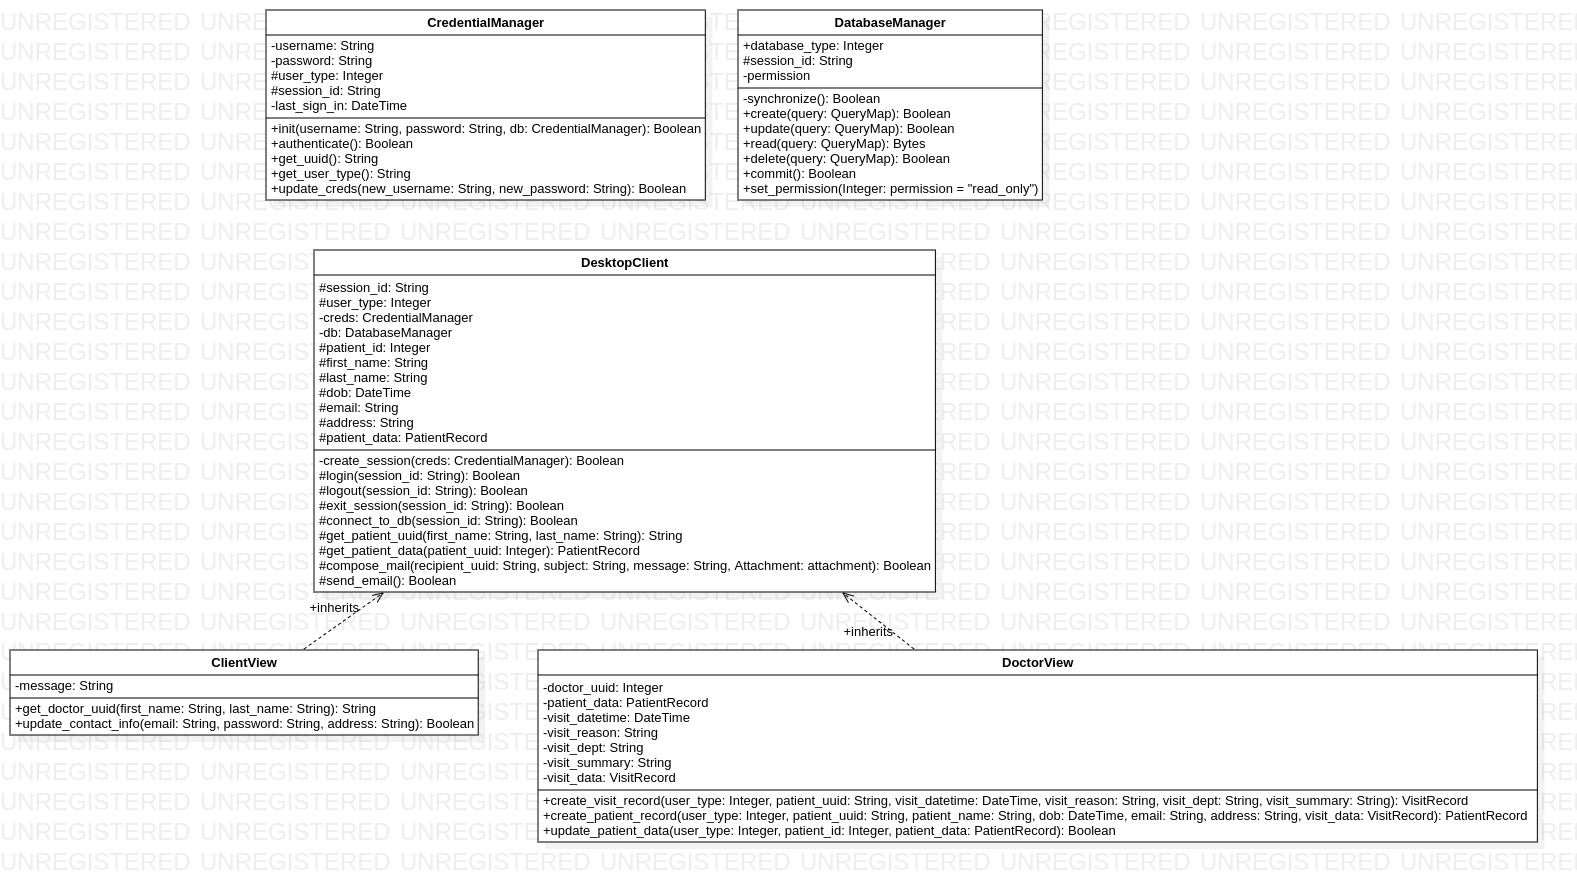
\includegraphics[width=\textwidth]{entity_classes.png}
    \caption{Entity Class Diagram}
    \label{fig:entity_classes}
    \addcontentsline{toc}{subsubsection}{Figure: Entity Class Diagram}
\end{figure}
\subsubsection{CredentialManager}
The \texttt{CredentialManager} class manages the user authentication and sessions. The class provides high-level access to authenticate user login information as well as update users' credentials. Its attributes \texttt{username} and \texttt{session\_id} are protected because they are shared amongst the classes that instantiate it. All the other attributes are private.

\subsubsection{DatabaseManager}
The \texttt{DatabaseManager} class manages the record classes defined in Figure \ref{fig:Record_class}. The class provides high-level access to create, read, update and read from all of the records in the system. Additional operations such as \texttt{commit()} and \texttt{set\_permission(permission: Integer)} are provided for additional security for the database.

\subsubsection{DesktopClient}
The \texttt{DesktopClient} class provides high-level access to interact with the \texttt{CredentialManager} and \texttt{DatabaseManager} classes. The class can be inherited by a user interface engine such as a graphical user interface or a web application.

\subsubsection{ClientView}
\subsubsection{DoctorView}

\begin{figure}[!htb]
    \centering
    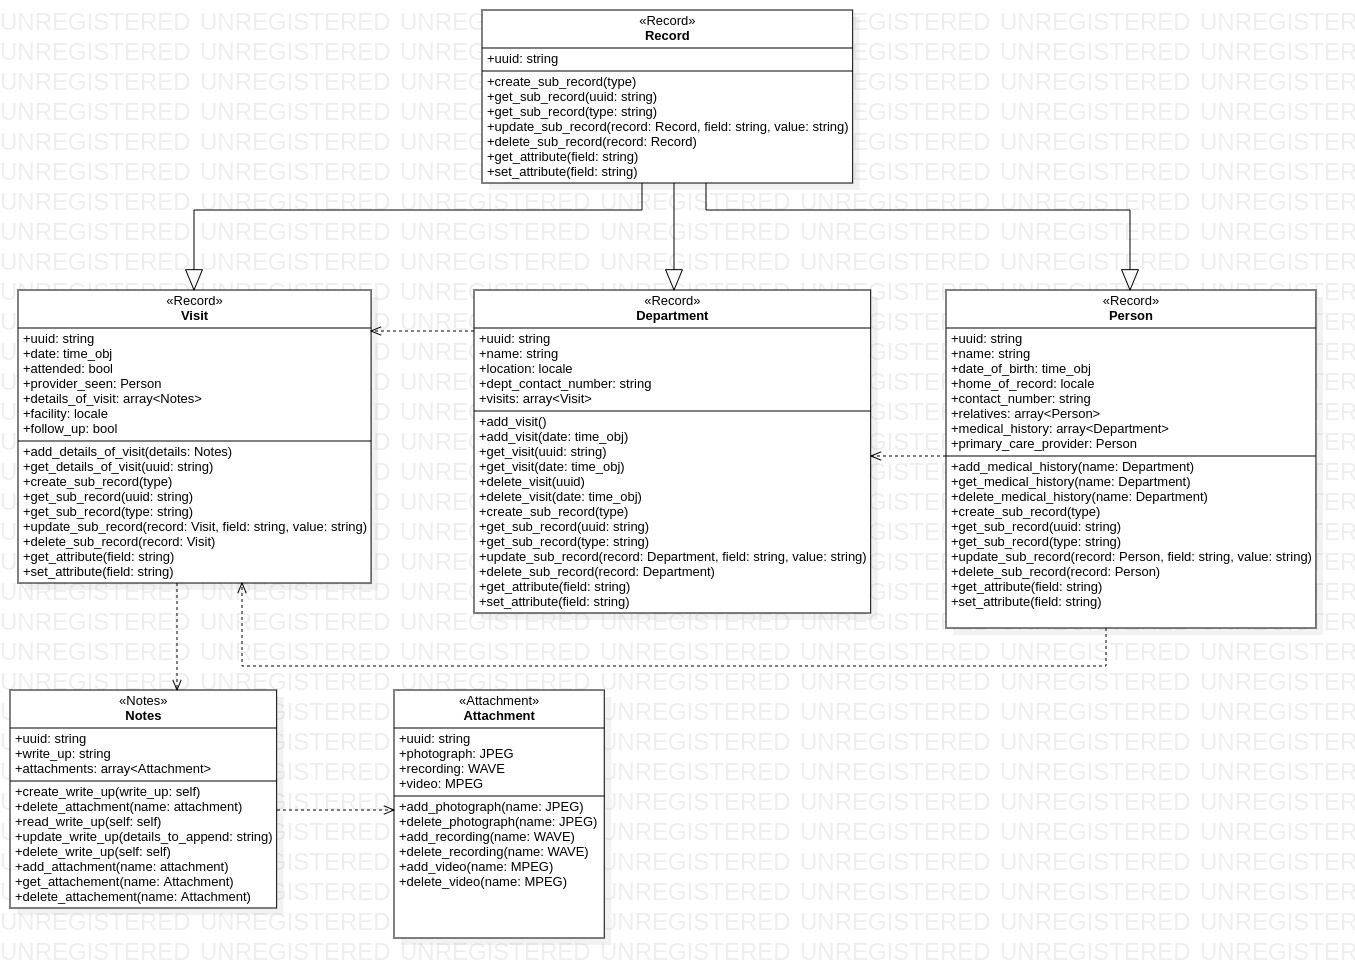
\includegraphics[width=\textwidth]{Record_class.jpg}
    \caption{Database/Record Class Diagram}
    \label{fig:Record_class}
    \addcontentsline{toc}{subsubsection}{Figure: Database/Record Class Diagram}
\end{figure}

\subsection{Pseudocode}
Some pseudocode of the major entity classes has been generated to demonstrate the design choices. The pseudocode snippets can be found in Appendix \ref{appendix:pseudocode}.

\newpage
\section{System Architecture}
\subsection{System Architecture Diagram}
The system architecture diagram of the deliverables draws everything together to show how different portions of the project work relate both in function and in scope. The system architecture diagram shows our different functions or processes on a horizontal axis and scope on the vertical axis, broad to narrow, with the roots being different actions the system might take-- considering our use case. Dependencies are shown with dotted arrows. Looking at the system architecture diagram in Figure \ref{fig:sys_arch_with_usecases} we can see that the system's function of updating a patients record depends on four components of the system: Database, Desktop Client, AdministrationSuite, and AuthenticationServer. Notice that this diagram also includes the interfaces for some of the components also. This demonstrates that in order to access more narrow in scope functions or capabilities one must access through that component's interface. Interfaces and their connections are also shown in Figure \ref{fig:components}.

\begin{figure}[!htb]
    \centering
    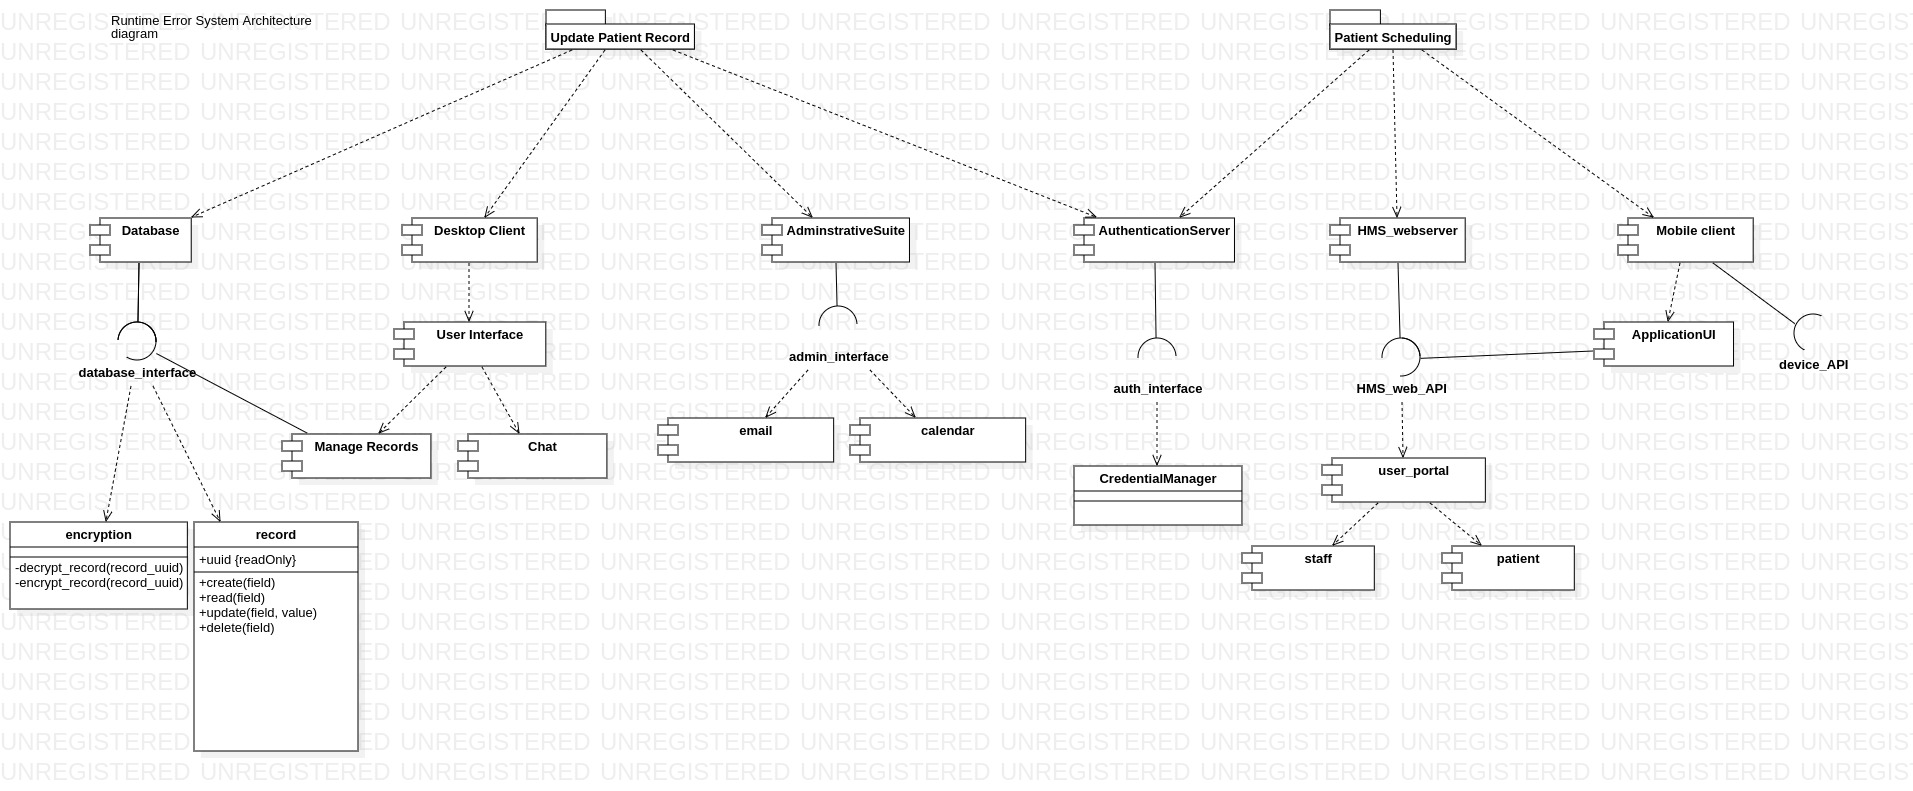
\includegraphics[width=\textwidth]{system_arch_with_usecases.jpg}
    \caption{System Architecture Diagram with use-cases as roots}
    \label{fig:sys_arch_with_usecases}
    \addcontentsline{toc}{subsubsection}{Figure: System Architecture Diagram}
\end{figure}
\clearpage
\newpage

\subsection{Component Diagram}
The components of the system are connected (networked, interface, etc) to create the GoodMead HMS. These connections are shown in Figure \ref{fig:components}. Each component is connected to other components through a port. This port is connected to some interface which allows it to communicate with other connected components. Consider the Authentication Server component. Three other component interact with it through its interface allowing them to create login sessions, verify credentials and access level (entitlements). Similarly with the Database.
The major components of the GoodMead HMS are the Cloud, Desktop Client, Administration Suite Server, Authentication Server, HMS WebServer, Mobile Client, Authentication Server, and Badge Reader. Part of the requirements were to have a Database hosted in the cloud and we can see that in our proposed system where the Database would be hosted. Additionally, we've included a Badge Reader component for additional security on desktop clients. The Mobile Client in the component diagram represents a mobile device which has the GoodMead mobile application (see: Appendix \ref{appendix:prototype}) installed to interact with the GoodMead HMS web server and services.


\begin{figure}[!htb]
    \centering
    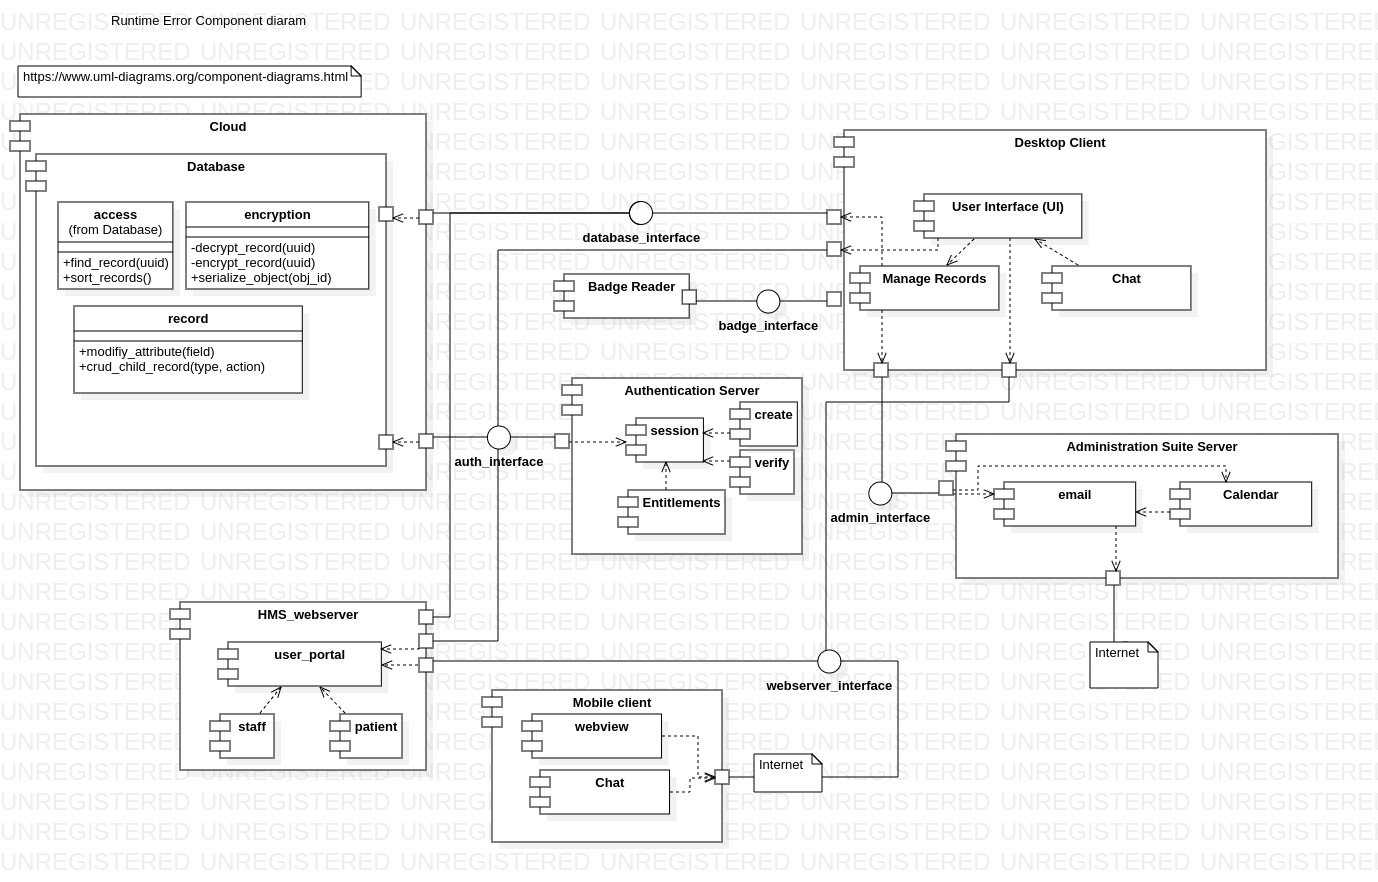
\includegraphics[width=\textwidth]{components.jpg}
    \caption{Component Diagram}
    \label{fig:components}
    \addcontentsline{toc}{subsubsection}{Figure: Component Diagram}
\end{figure}
\clearpage
\newpage

\subsection{Component Entity Mapping}
The component to entity class mapping allows us, at a glance to verify which components are linked and directly relevant to which entity classes (see: Figures \ref{fig:entity_classes} and \ref{fig:Record_class}). Most of the components have at least one entity class that it maps to that describes its behaviour at a high level (attributes and functions). There are two components that do not have entity classes that map to them: Mobile Client and Badge Reader. For the Badge Reader we envision a third-party source providing this solution. The Mobile Client component utilizes the Client View entity class which is served by the HMS WebServer. The component with the most entity classes is the Cloud portion of the system. This is because we utilize a database class on the cloud which manages interactions with the records and multiple record classes which demonstrate the complexity that would be required in a hospital records system. 

\begin{figure}[!htb]
    \centering
    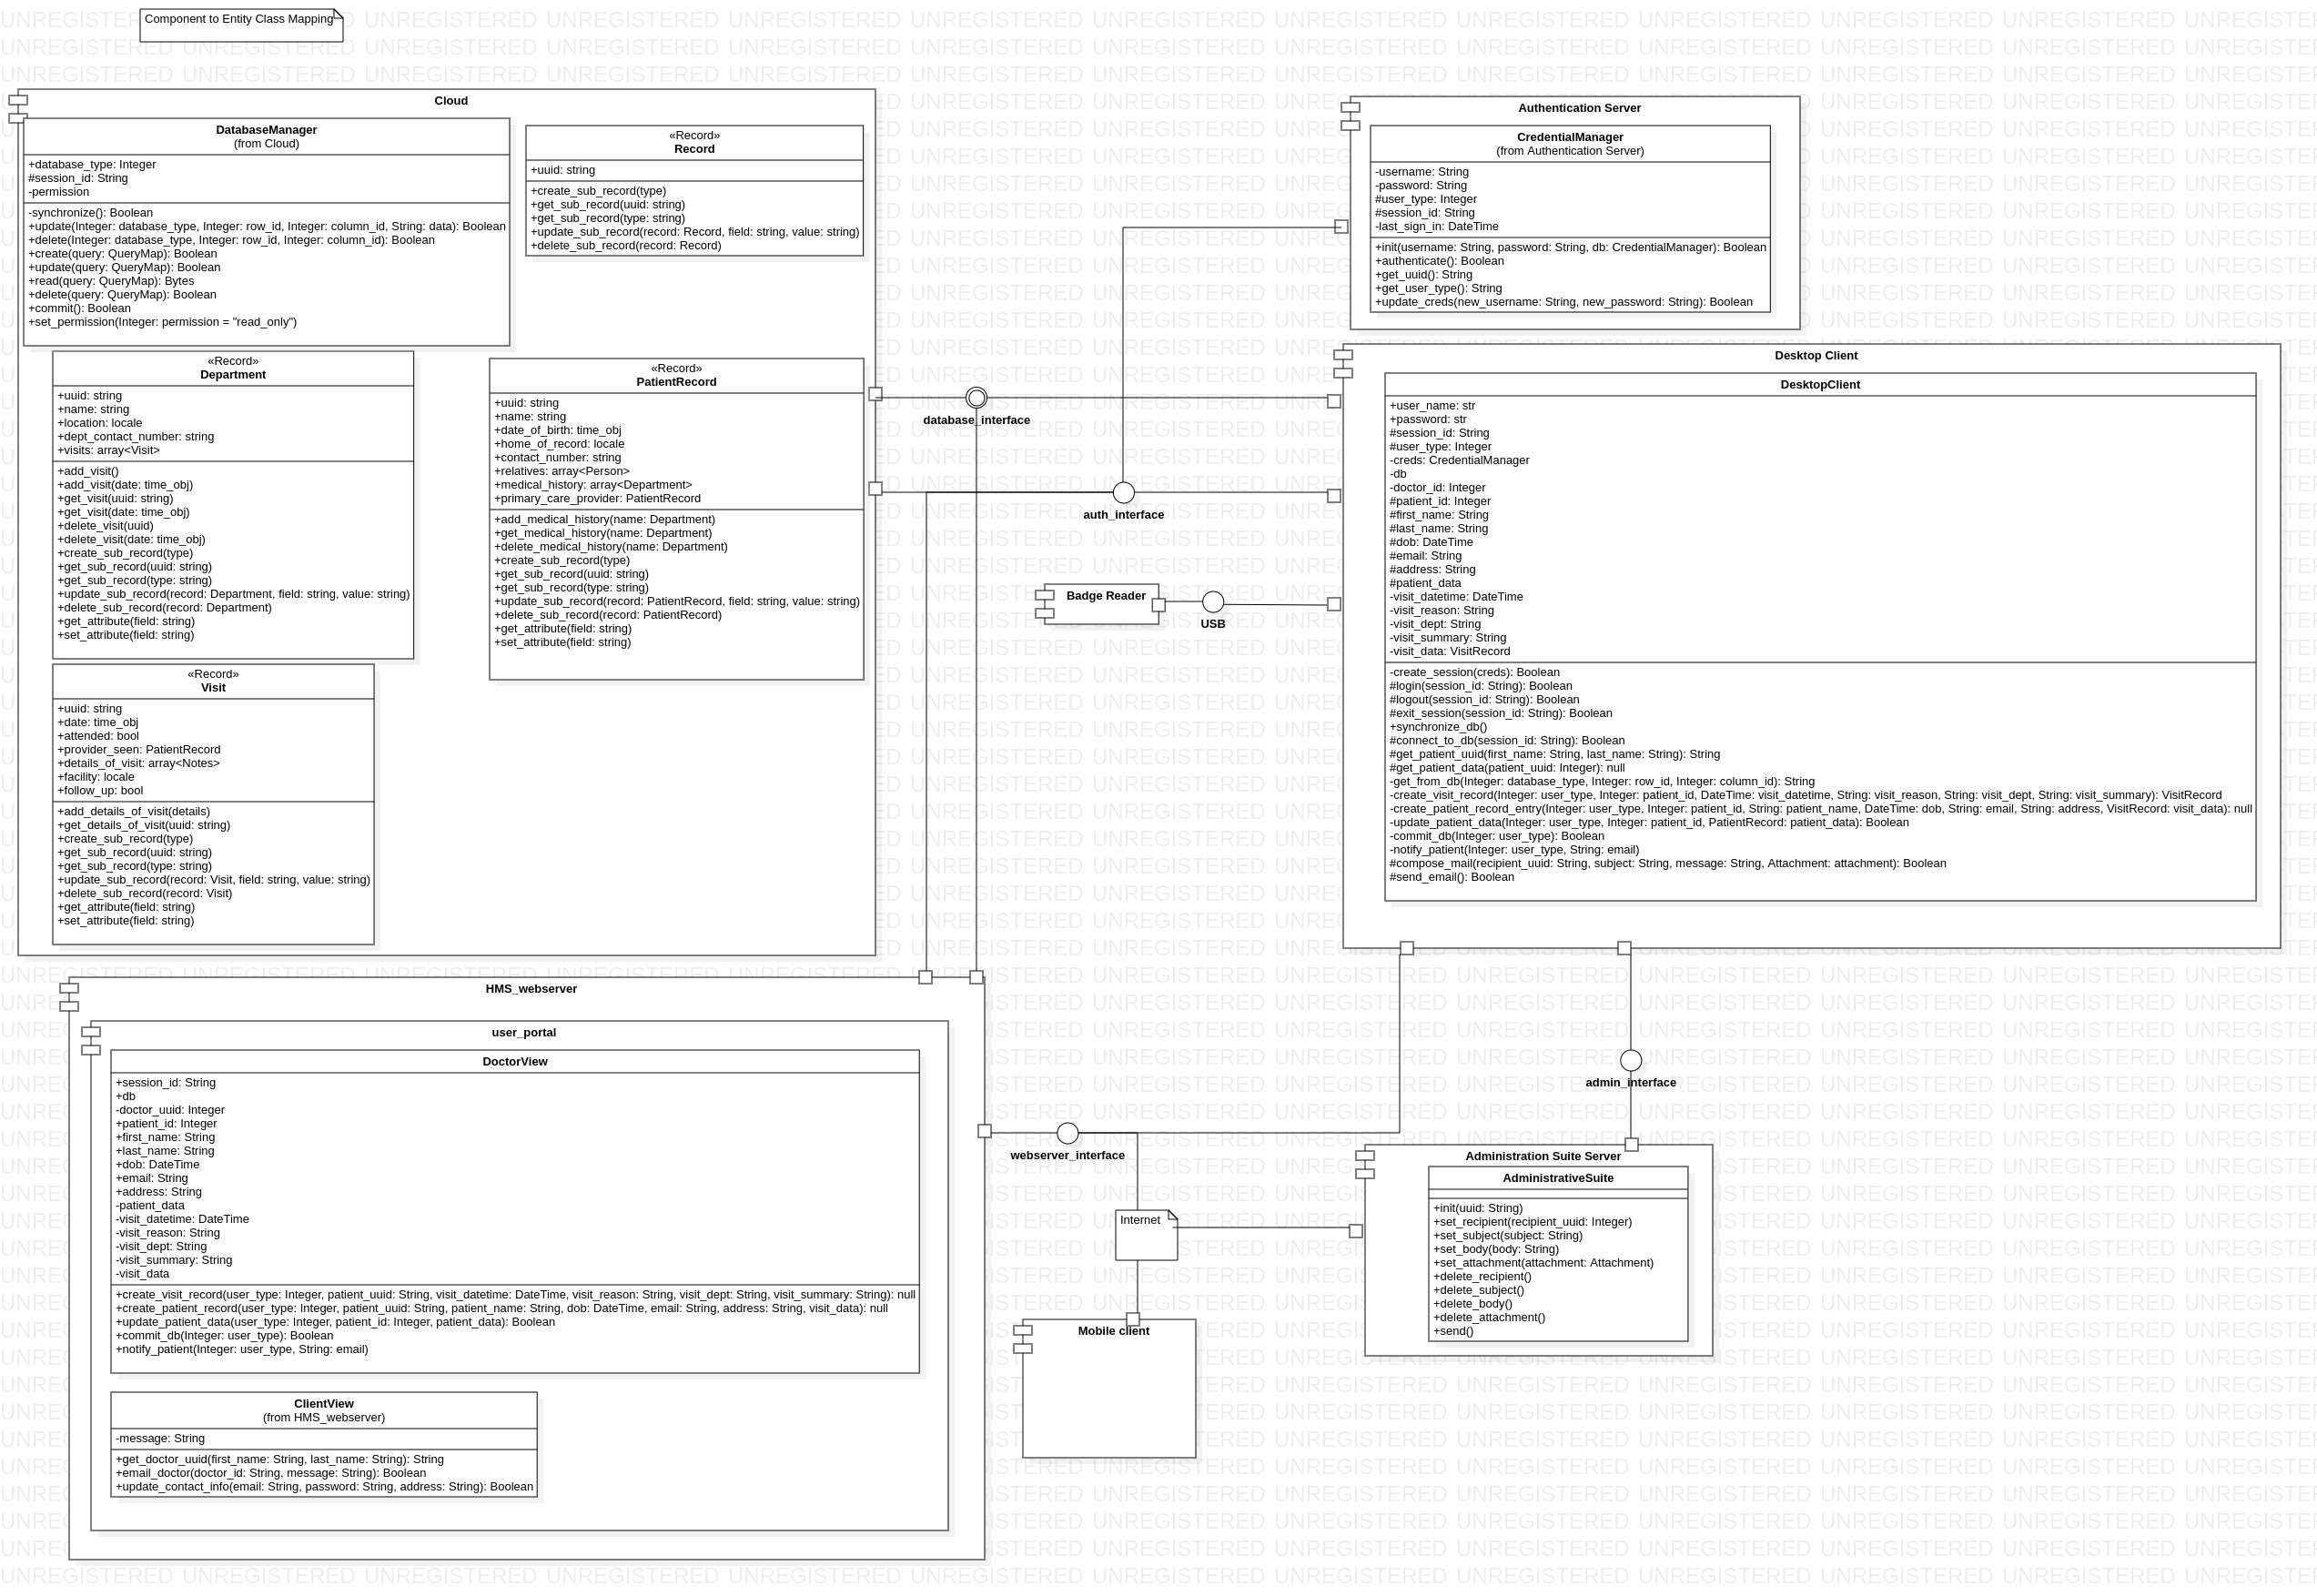
\includegraphics[width=\textwidth]{component_and_entity_classes.jpg}
    \caption{Component-Entity Class Map}
    \label{fig:components_and_entity_classes}
    \addcontentsline{toc}{subsubsection}{Figure: Component-Entity Class Map}
\end{figure}

\subsection{UI Flow}
This UI Flow corresponds to the Activity Diagram from the perspective of the Patient Actor using a mobile device with the GoodMead application installed. The patient is an existing patient with a previously registered account with GoodMead Hospital.

\begin{enumerate}
    \item Patient opens the GoodMead app
    \item Patient logs in using credentials they established when they first became a GoodMead patient
    \item Patient views their Profile page and checks their listed information
    \item Patient taps on the Records link from Dashboard
    \item Patient views a list of their Visit Records with GoodMead Hospital and taps on the latest Record, which has a Notification icon marking it as recently edited
    \item Patient views the Record from their recent Optometry appointment. The doctor in the Activity Diagram had added Patient Visit Notes to the Record, which the patient can see marked as new with a Notification Icon
    
\end{enumerate}

\addcontentsline{toc}{subsubsection}{Figure: UI Flow}
\includepdf[pages={1-}, nup=2x1, frame=true, delta=4 4, offset=3 3]{ActivityUI.pdf}

\clearpage
\newpage
\begin{appendices}
\section{Code snippets} \label{appendix:pseudocode}
\begin{pseudocode}[caption={CredentialManager Entity Class}, label={creds}]
class CredentialManager {

  operation init(username: String, password: String, db: CredentialManager) -> Boolean {
    assign attribute username = encrypt(username)
    assign attribute password = encrypt(password)
    assign attribute db = dereference(db)
    call db.synchronize()
    if no errors raised {
      return true
    } else {
      return false
    }
  }

  operation authenticate() -> Boolean {
    call db.read(Integer: database_type = PatientRecord, username: Bytes = username, password: Bytes = password)
    if return value is true {
      assign attribute uuid = return value uuid
      assign attribute user_type = return value user_type
      return true
    } else {
      return false
    }
  }

  operation get_uuid() -> String {
    return attribute uuid
  }

  operation get_user_type() -> String {
    return attribute user_type
  }

  operation update_creds(new_username: String, new_password: String) -> Boolean {
    if user_type is valid {
      call db.set_permission(Integer: mode = "read_write")
      call db.update(Integer: database_type = PatientRecord, username: Bytes = new_username, password: Bytes = new_password)
      call db.set_permission(Integer: mode = "read_only")
      return true
    } else {
      return false
    }
  }

}
\end{pseudocode}

\begin{pseudocode}[caption={CredentialManager Entity Class}, label={db}]
class DatabaseManager {

  operation synchronize() -> Boolean {
    open database and assign to attribute db
    synchronize db
    assign attribute permission to "read_only"
    if no errors raised {
      return true
    } else {
      return false
    }
  }

  operation create(query: QueryMap) -> Boolean {
    check if attribute permission is valid {
      parse and convert query into valid executable database query
      call db.create(query)
      if no errors raised {
        return true
      } else {
        return false
      }
    }
  }

  operation read(query: QueryMap) -> String {
    parse and convert query into valid executable database query
    call db.read(query)
    if no errors raised {
      convert return value to String
    } else {
      return empty string
    }
  }

  operation update(query: QueryMap) -> Boolean {
    check if attribute permission is valid {
      parse and convert query into valid executable database query
      call db.update(query)
      if no errors raised {
        return true
      } else {
        return false
      }
    }
  }

  operation delete(query: QueryMap) -> Boolean {
    check if attribute permission is valid {
      parse and convert query into valid executable database query
      call db.delete(query)
      if no errors raised {
        return true
      } else {
        return false
      }
    }
  }

  operation commit() -> Boolean {  
    call db.commit()
    if no errors raised {
      return true
    } else {
      return false
    }
  }

  operation set_permission(Integer: permission = "read_only"){
    assign attribute permission = permission
  }

}
\end{pseudocode}

\begin{pseudocode}[caption={DesktopClient Entity Class}, label={desktop}]
class DesktopClient {

  operation create_session(creds: CredentialManager) -> Boolean {
    instantiate CredentialManager object: creds
    call creds.init(username: String, password: String, reference_to(db): CredentialManager)
    call creds.authenticate()
    while return value is false {
      call creds.init(username: String, password: String, reference_to(db): CredentialManager)
      if return value is true {
        assign session_id = creds.get_session_id()
        assign user_type = creds.get_user_type()
        return true
      }
    }
  }

  operation connect_to_db(session_id: String) -> Boolean {
    instantiate DatabaseManager object: db
    call db.synchronize()
    call db.create(database_type: Integer = logs, session_id: String, last_login: DateTime = time.now())
  }

  operation get_patient_uuid(first_name: String, last_name: String) -> String {
    call db.read(database_type: Integer = PatientRecord, first_name: String = first_name, last_name: String = last_name)
    return the return value
  }

  operation get_patient_data(patient_uuid: Integer) -> PatientRecord {
    call db.read(database_type: Integer = PatientRecord, patient_uuid: String = patient_uuid)
    return the return value
  }

  operation compose_mail(recipient_uuid: String, subject: String, message: String, Attachment: attachment) {
    instantiate AdministrativeSuite object: admin
    call admin.init(uuid: String)
    call admin.set_recipient(recipient_uuid: String)
    call admin.set_subject(subject: String)
    call admin.set_body(body: String)
    call admin.set_attachment(attachment: Attachment)
  }

  operation send_email() -> Boolean {
    call admin.send()
    return the return value
  }
}
\end{pseudocode}

\begin{pseudocode}[caption={DoctorView Derived Entity Class}, label={doctor}]
class DoctorView inherits from DesktopClient {

  operation create_visit_record(user_type: Integer, patient_uuid: Integer, visit_datetime: DateTime, 
    visit_reason: String, visit_dept: String, visit_summary: String) -> VisitRecord {
    convert parameters to VisitRecord object
  }

  operation create_patient_record(user_type: Integer, patient_uuid: String, patient_name: String,
    dob: DateTime, email: String, address: String, visit_data: VisitRecord) -> PatientRecord {
    convert parameters to PatientRecord object
  }

  operation update_patient_data(user_type: Integer, patient_id: String, patient_data: PatientRecord) -> Boolean {
    call db.update(database_type: Integer = PatientRecords, user_type: Integer = user_type,
      patient_id: Integer = patient_id, patient_data: PatientRecord = patient_data)
    call db.commit()
    call compose_mail(recipient_uuid: String = patient_uuid, subject: String = "Record updated",
      message: String = "Dear patient, your records have been updated.\n")
    call send_mail()
    return the return value
  }

}
\end{pseudocode}
\begin{pseudocode}[caption={ClientView Derived Entity Class}, label={client}]
class ClientView inherits from DesktopClient {

  operation get_doctor_uuid(first_name: String, last_name: String) -> String {
    call db.read(database_type: Integer = DoctorRecords, first_name: String = first_name, last_name: String = last_name)
    return the return value
  }

  operation update_contact_info(email: String, password: String, address: String) -> Boolean {
    call create_patient_record(user_type: Integer, patient_uuid: Integer, email: String, address: String)
    save reference to return object
    call update_patient_data(user_type: Integer, patient_id: Integer, patient_data: PatientRecord)
  }

}
\end{pseudocode}

\newpage
\section{Mobile Application Prototype}

\label{appendix:prototype}
\includepdf[pages={1-}, nup=2x1, frame=true, delta=4 4, offset=3 3]{UIPrototype.pdf}

\end{appendices}

\end{document}
